\chapter{Entorno de Trabajo}\label{cap:07entorno}
Este capítulo se divide en cinco secciones \ref{sec:07intro} Introducción, \ref{sec:07estandares} Estándares de OHDSI, \ref{sec:07herramientas} Herramientas de OHDSI, \ref{sec:07programas} Programas informáticos empleados y \ref{sec:07conclusiones} Conclusiones.

\section{Introducción}\label{sec:07intro}

En este capítulo se presenta el entorno de trabajo utilizado durante el desarrollo del proyecto. Consiste principalmente en la utilización de los estándares y herramientas que provee OHDSI para conducir estudios observacionales.

\textbf{No se puede entender la herramienta ATLAS sin entender el ecosistema de herramientas y estándares OHDSI que la acompañan}.

Por tanto, en la sección \ref{sec:07estandares} ''Estándares de OHDSI'' se presentan los dos estándares fundamentales: el Modelo de Datos Común de OMOP y el Vocabulario.

En la sección \ref{sec:07herramientas} ''Herramientas de OHDSI'' se presenta el conjunto de herramientas que ofrece la organización, prestando especial atención a la herramienta ATLAS.

Por último, en la sección \ref{sec:07programas} ''Programas informáticos empleados'' se presentan los programas informáticos utilizados para desplegar el entorno de trabajo del proyecto.


\section{Estándares de OHDSI}\label{sec:07estandares}

%\subsection{Estandarización de los datos} \label{subsec:05estandarDatos}

En términos de estandarización, OHDSI realiza una labor muy importante para paliar las dificultades de la investigación con datos de salud a causa de la heterogeneidad de los datos y estudios. Debido a la amplia colaboración internacional de la organización se recocone la necesidad de estándares que permitan el intercambio de información sin pérdida entre los distintos sistemas de información de los miembros de la comunidad.

OHDSI ofrece dos estándares: el Modelo de Datos Común de OMOP y el Vocabulario. A continuación se describe cada uno de ellos en mayor detalle.

%La estandarización de la investigación en OHDSI se realiza en dos planos: a nivel de datos y a nivel de investigación. La estandarización a nivel de datos se realiza a través del uso del Modelo de Datos Común y el Vocabulario y la estandarización a nivel de investigación mediante la ''investigación metodológica''. A continuación se describe en una subsección cada uno de estos estándares.

\subsection{Modelo de Datos Común de OMOP} \label{subsec:07cdm}

El Modelo de Datos Común o \textit{Common Data Model (CDM)} de OMOP es ''un estándar de datos comunitario abierto, diseñado para estandarizar la estructura y el contenido de los datos de observación y permitir análisis eficientes que puedan producir evidencia confiable'' \cite{gitPagesCMD}, en definitiva, es un modelo semántico estándar para estructurar los datos de salud. La información más relevante y actualizada sobre el CDM se encuentra en su página de github \cite{gitPagesCMD} y en el capitulo 4 del Libro de OHDSI \cite{OHDSIbook}.

\subsubsection{Características}

El modelo de datos de OMOP presenta características importantísimas para hacer frente a las necesidades del panorama socio-sanitario actual presentado en la sección \ref{sec:01Contexto} ''Marco Contextual''. A continuación se presentan las características más relevantes del modelo (extraídas de la sección  4.1 del Libro de OHDSI \cite{OHDSIbook}), según las necesidades identificadas previamente.

\begin{itemize}
    \item \textbf{Estructura diseñada para la investigación}. 
    El modelo presenta una estructura única y óptima para un propósito concreto: el de facilitar la realización de estudios observacionales. Por tanto reduce notoriamente los desafíos relativos a las diferentes estructuras y propósitos con los que se recogen los datos clínicos.
    \item \textbf{Modelo centrado en el paciente}. Es un modelo centrado en el paciente (alineado con la misma característica de la Sanidad 4.0). Estructuralmente esto significa que todos los eventos y tablas están relacionados con la tabla central del paciente, denominada \textit{Person}. 
    \item \textbf{Protección y privacidad}. El modelo limita el acceso a la información personal de los pacientes, evitando en la medida de lo posible el acceso a información personal sensible como nombres o apellidos, para fomentar la protección y privacidad de los datos. Mayor información sobre las técnicas empleadas para ello se encuentran en el apartado \textit{Privacidad del paciente y OMOP} de la página de github \cite{gitPagesCMD}.
    \item \textbf{Reutilización de estándares}. Un aspecto importantísimo es que el modelo propone su propio estándar pero sin olvidar los estándares globalmente utilizados, de manera que integra y reutiliza los conceptos provenientes de estándares ya existentes (ej. SNOMED, LOINC...) referenciándolos en su propio Modelo de Datos Común. El conjunto de todos los estándares conforma el Vocabulario.
    \item \textbf{Neutralidad tecnológica}. El modelo no requiere una tecnología específica sino que puede estructurarse en cualquier base de datos relacional (ej. Oracle, SQL Server...), ajustándose a los requisitos tecnológicos necesarios de cada organización.
    
\end{itemize}

\subsubsection{Modelo de Datos Lógico}

Actualmente el CDM ha lanzado ya su sexta versión, sin embargo, esta aún no está soportada por todas las herramientas de la comunidad, por lo que se sigue sugiriendo el uso del CDM v5.4 o 5.3 indistintivamente, que son las últimas versiones completamente funcionales. 

A la hora de realizar un estudio en ATLAS o cualquier otra herramienta del ecosistema OHDSI la base de datos estará necesariamente estandarizada a este modelo por lo que es importante conocer su estructura fundamental. A continuación, en la Figura \ref{fig:cdm54} ''Estructura del CDM v5.4'' se presenta la estructura lógica de este modelo y en la Figura \ref{fig:cdm_ER} ''Modelo Entidad-Relación del CDM v5.4'', la estructura del modelo Entidad-Relación. Adicionalmente existe una página web que proporciona un modelo interactivo para facilitar su estudio \cite{CDMinteractive}.

Aunque el modelo de datos común de OMOP es muy complejo, incluso existen grupos de trabajo de la comunidad (\textit{workshops}) especializados sólo en este ámbito, en esta subsección del trabajo tan solo se van a presentar los conceptos considerados estrictamente necesarios para la comprensión del contenido del mismo.

\begin{figure}[H]
    \centering
    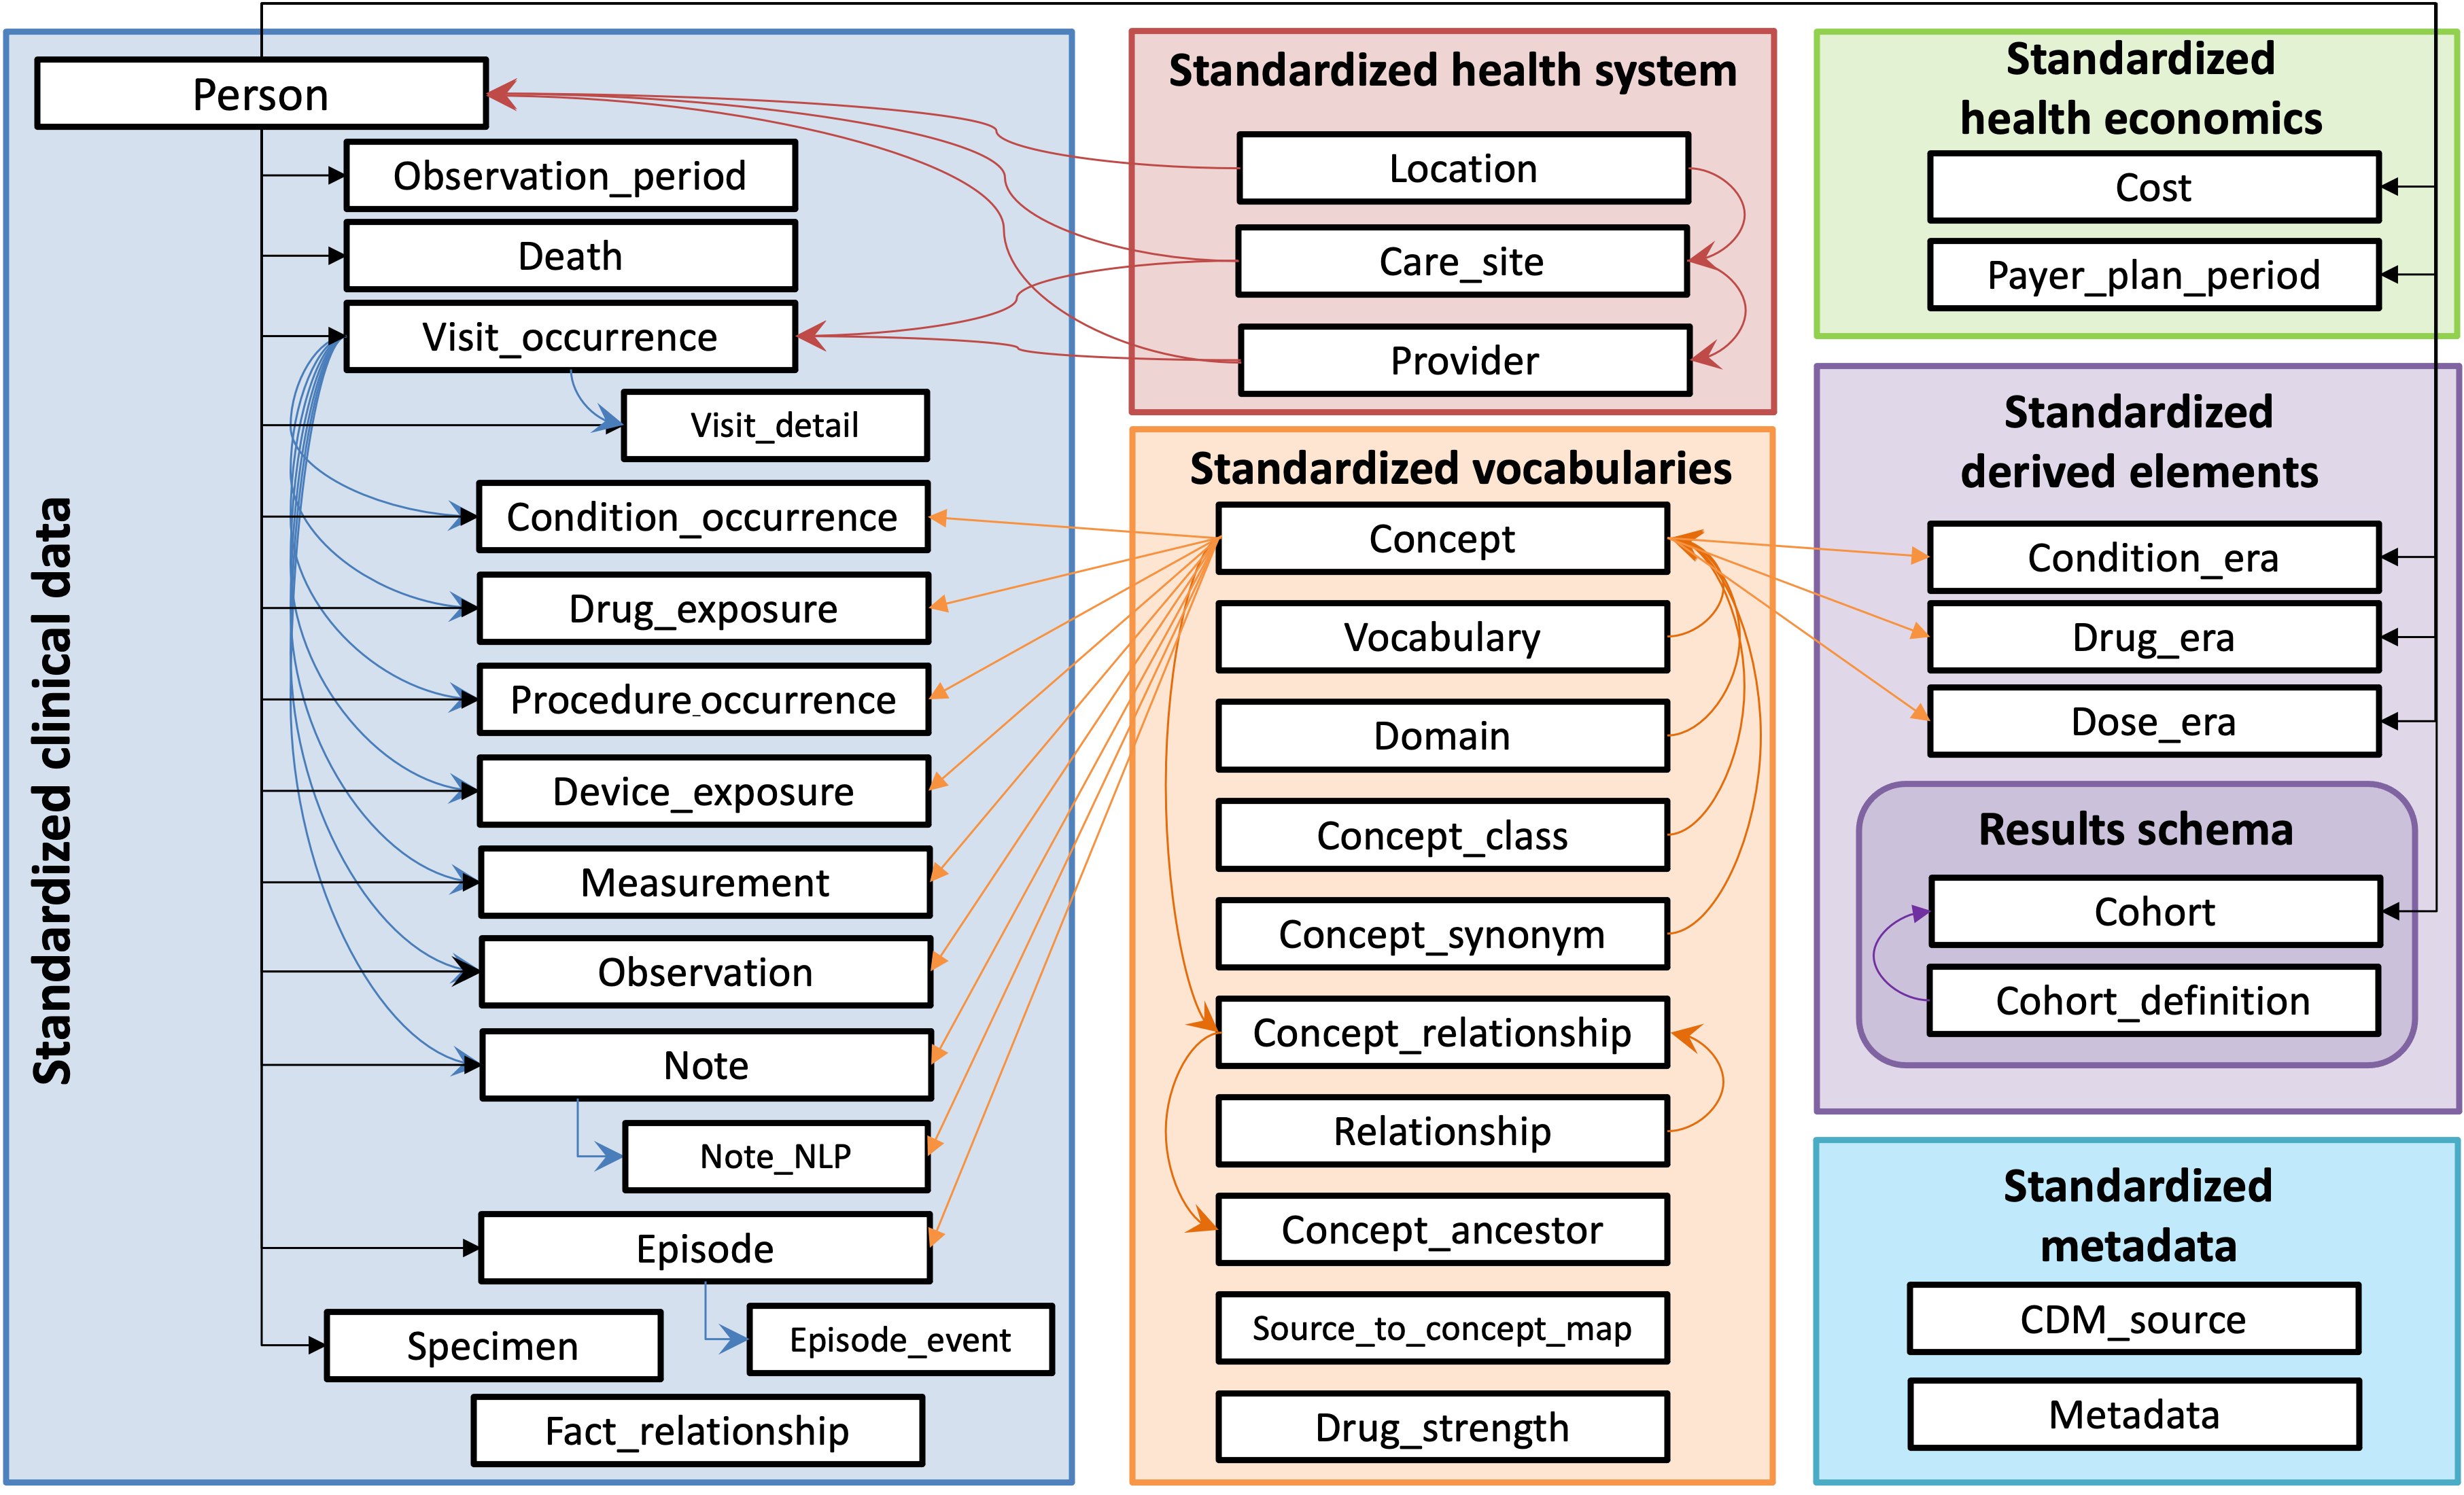
\includegraphics[width=0.90\textwidth]{figures/cdm54.png}
     \caption{Estructura del CDM v5.4. Extraída de la página de github del CDM \cite{gitPagesCMD}}
    \label{fig:cdm54}
\end{figure}

\begin{figure}[H]
    \centering
    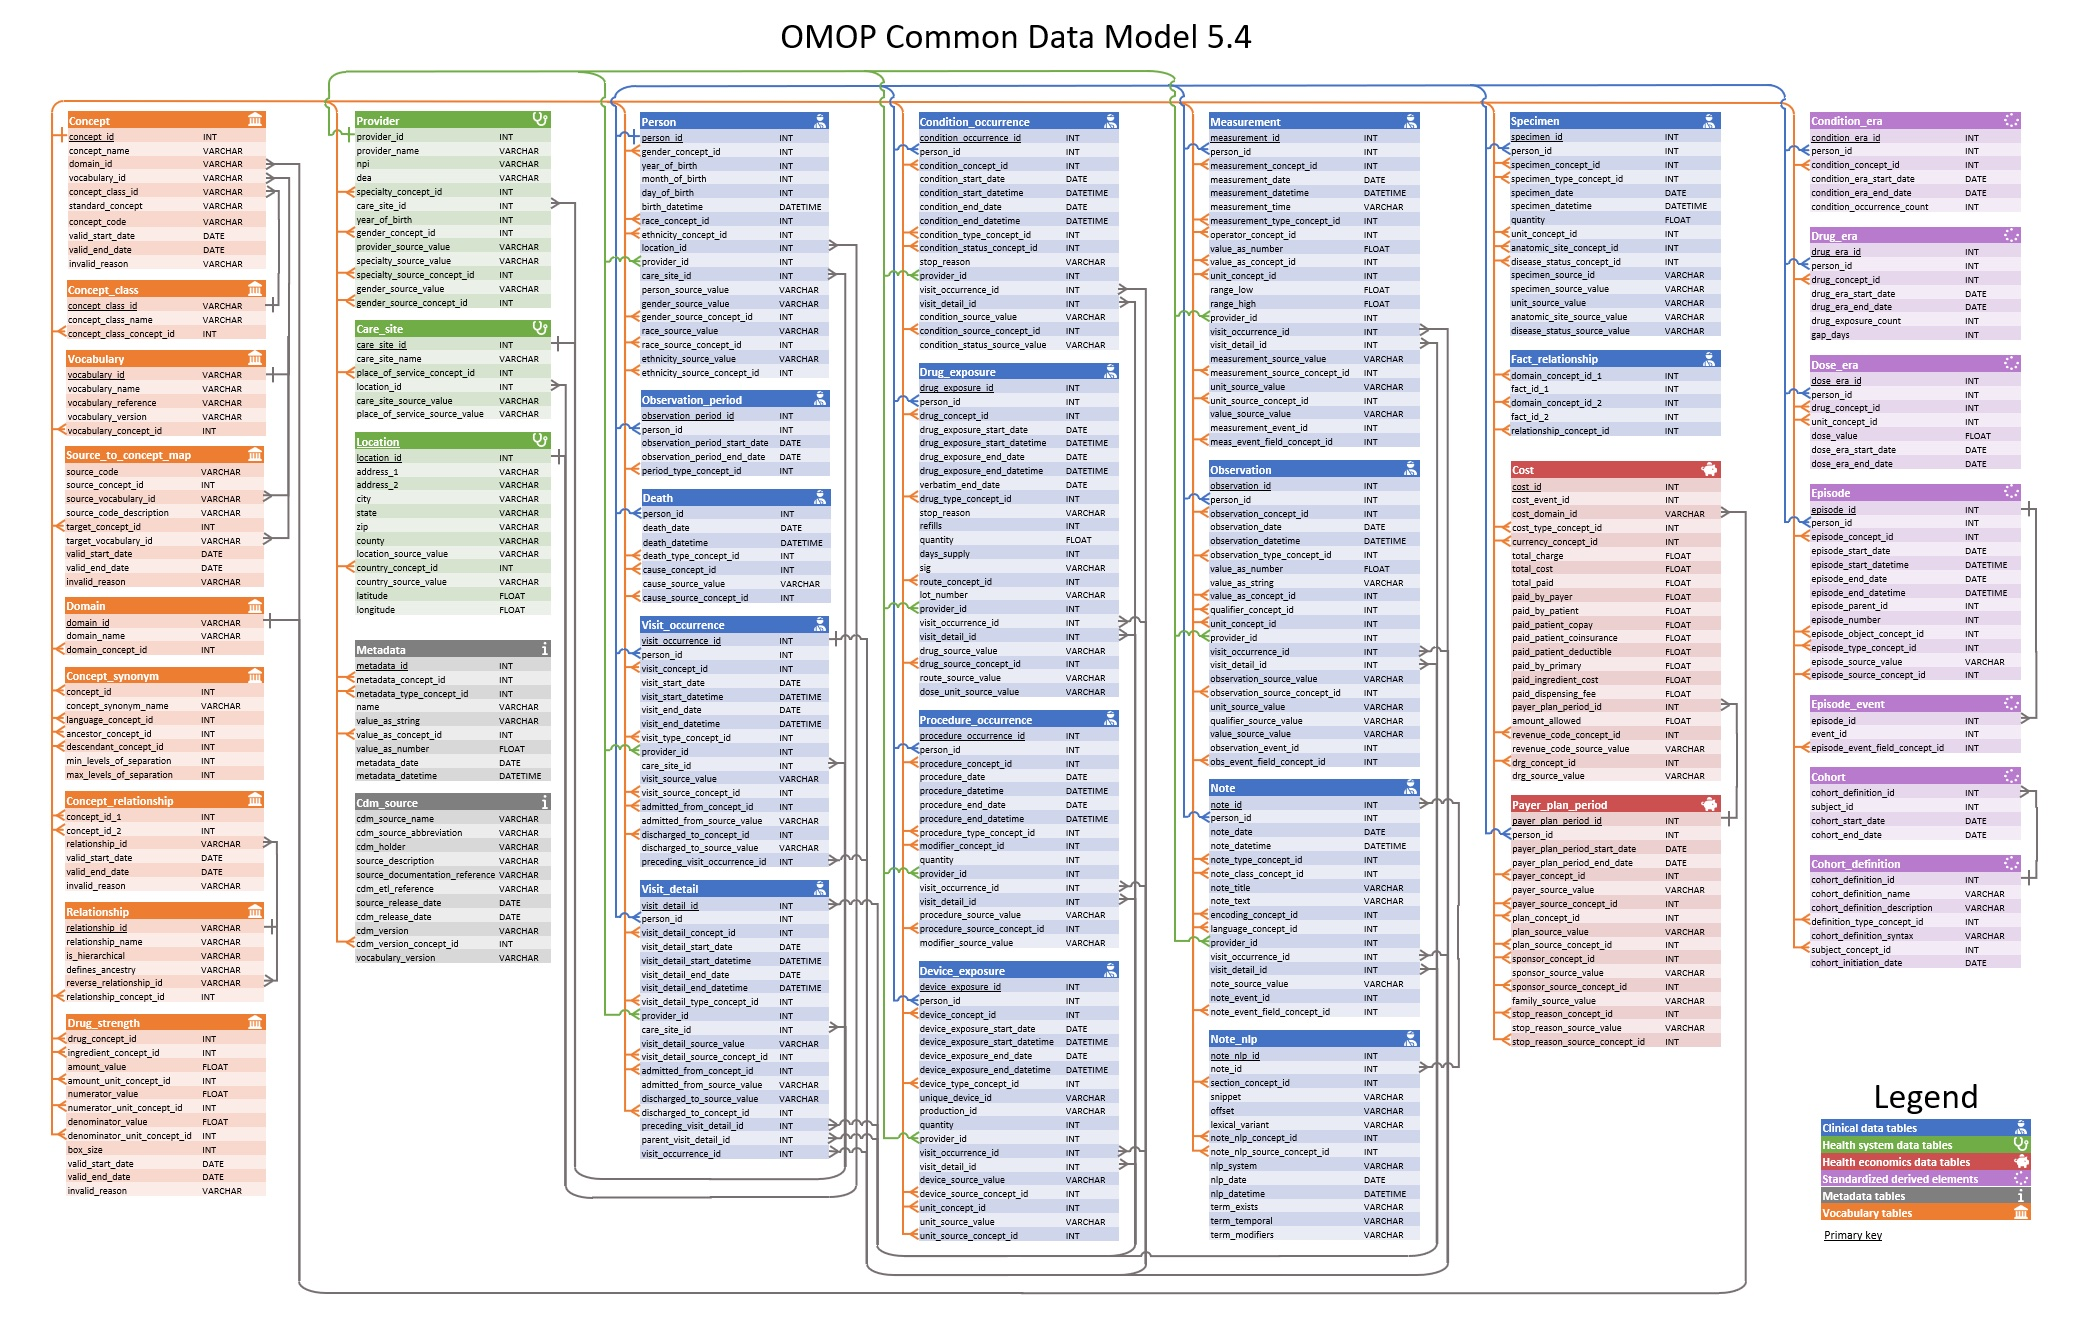
\includegraphics[width=1\textwidth]{figures/cdm_ER.jpg}
     \caption{Modelo Entidad-Relación del CDM v5.4. Extraída de la página de github del CDM \cite{gitPagesCMD}}
    \label{fig:cdm_ER}
\end{figure}

El modelo se comprende de 39 tablas agrupadas en seis grupos, de los cuales se destaca la importancia de tres: Datos clínicos estandarizados (\textit{Standardized clinical data}, en azul), Vocabularios estandarizado (\textit{Standardized vocabularies}, en naranja) y Elementos derivados estandarizados (\textit{Standardized derived elements}, en morado). El grupo más importante es el de datos clínicos, que contiene la tabla Persona (\textit{Person}), por la característica centrada en el paciente del modelo.

Cada evento clínico se registra en el modelo como un \textbf{Concepto} (\textit{Concept}), perteneciente al grupo del Vocabulario estandarizado (en naranja). Además, cada concepto está ligado a un \textbf{Dominio} que especifica a qué tipo de información clínica corresponde dicho concepto. A continuación se muestra una tabla con los 30 dominios existentes y la cantidad de conceptos que tiene asociado cada uno.

\begin{figure}[H]
    \centering
    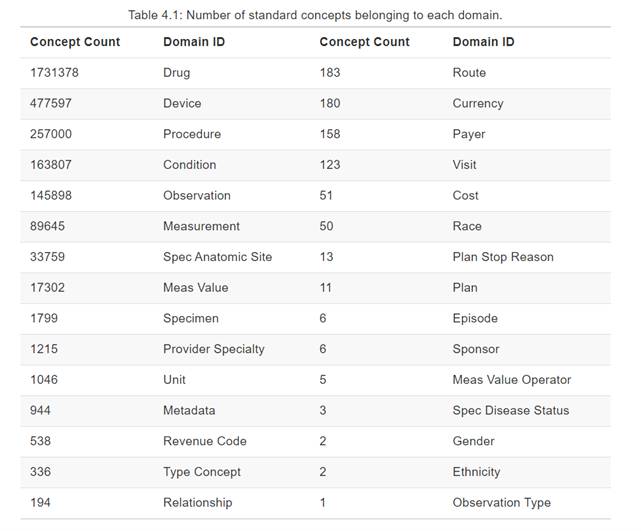
\includegraphics[width=0.80\textwidth]{figures/cdm_domains.png}
     \captionof{table}{Dominios del CDM v5.4. Extraída del Libro de OHDSI \cite{OHDSIbook}}
    \label{fig:cdm_domains}
\end{figure}

La información que contiene cada dominio se puede inferir fácilmente de la traducción al español del nombre por lo que no se va a hacer hincapié en ello. No obstante, se puede encontrar más información en \cite{OHDSIbook}, \cite{gitPagesCMD} o \cite{CDMinteractive}.

\subsection{Vocabulario}\label{subsec:07vocab}

El Vocabulario es otro de los elementos centrales del Modelo de Datos Común de OMOP y una gran herramienta de estandarización e interoperabilidad entre sistemas. Como se ha comentado en varias ocasiones, actualmente hay muchos estándares distintos en funcionamiento que establecen las terminologías de los eventos clínicos (por ejemplo LOINC, SNOMED CT, RxNorm...). El beneficio del Vocabulario de OMOP es que integra todos los vocabularios ya existentes en un único \textbf{Vocabulario estándar}, a través de la referenciación entre \textbf{conceptos estándar} (pertenecientes a OMOP) y conceptos no estándar (pertenecientes a vocabularios alternativos).

El Vocabulario de OHDSI, por tanto, impera sobre un conjunto de vocabularios, respetando las diversas procedencias de cada término pero mapeándolos a un único vocabulario estándar. \textbf{Cada concepto no estándar está asociado a un concepto estándar} y esta es la clave del Vocabulario. 

Como todas las herramientas de la comunidad, la información acerca de este está disponible online de forma pública en el capítulo 5 del Libro de OHDSI \cite{OHDSIbook} y en la página de github del CDM \cite{gitPagesCMD}. Por otra parte, existe un buscador online de términos en el Vocabulario de OMOP denominado ATHENA \cite{ATHENAweb}. 

\begin{figure}[H]
\centering
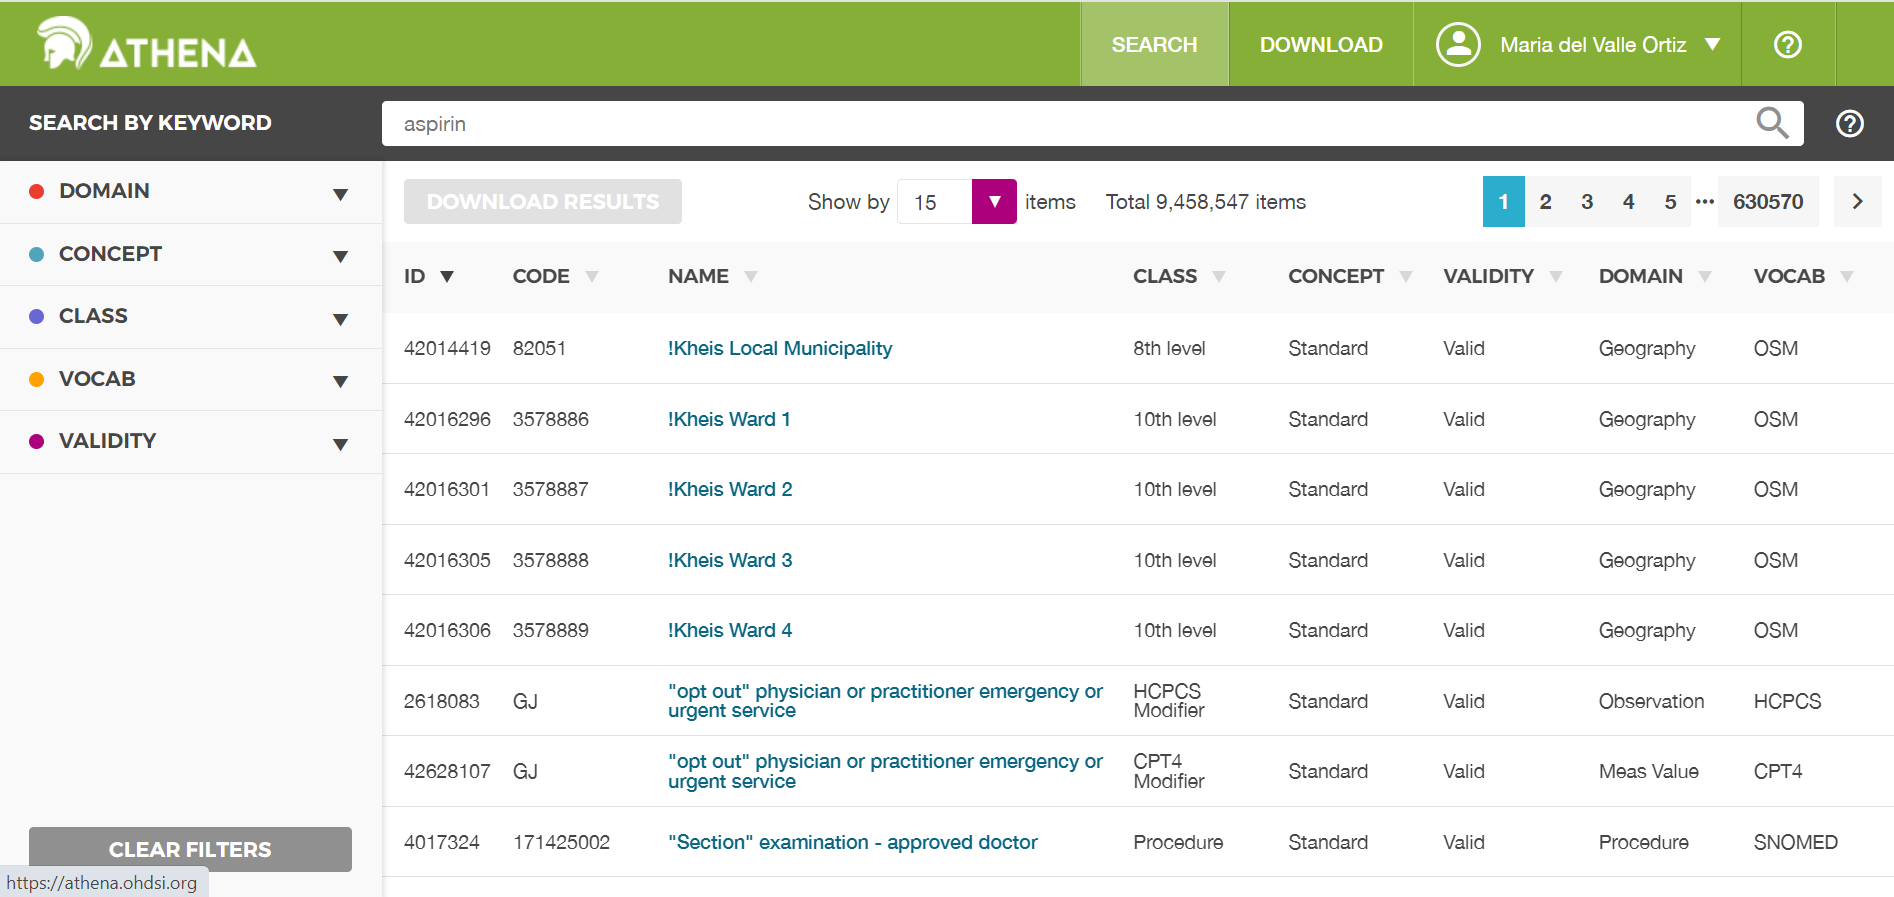
\includegraphics[width=0.90\textwidth]{figures/ATHENAcap.png}
     \caption{Captura de pantalla del menú principal de ATHENA}
    \label{fig:ATHENAcap}
\end{figure}

Actualmente hay más de nueve millones de términos registrados en el Vocabulario de OMOP, como se muestra en la Figura \ref{fig:ATHENAcap} ''Captura de pantalla del menú principal de ATHENA'', y 155 vocabularios distintos coexisten juntos en el estándar, de los cuales al menos 30 son vocabularios internos de OMOP.

%\textcolor{red}{- lA RELACIÓN QUE GUARDAN LOS CONCEPTOS ENTRE SÍ ES JERARQUICA}

\section{Herramientas de OHDSI} \label{sec:07herramientas}

OHDSI proporciona un conjunto de herramientas para facilitar la realización de los estudios e investigaciones a raíz de los datos clínicos y fomentar la interoperabilidad entre estos, aportando un estándar de herramientas. 

Las herramientas que proporciona la organización están disponibles públicamente online y de forma gratuita y son desarrolladas por los propios miembros de la comunidad. Entre todas las herramientas, para la realización de este proyecto se destaca la herramienta de análisis de datos clínicos ATLAS, aunque también existen otras herramientas importantes de forma indirecta que se describen a continuación.

\subsection{ATLAS} \label{subsec:07ATLAS}

ATLAS es la herramienta de OHDSI por excelencia porque es la que estandariza el análisis observacional una vez que la base de datos está convertida al modelo OMOP. La documentación oficial sobre ATLAS se encuentra en el capítulo 8 del Libro de OHDSI y en su repositorio de github \cite{githubATLAS}. Además, aparte de la documentación oficial, hay montones de información esparcidas por la red sobre ATLAS, en publicaciones científicas, foros de OHDSI, videotutoriales en youtube y un largo etcétera.

\begin{figure}[H]
\centering

\includegraphics[width=0.25\textwidth]{figures/ATLASlogo.png}
     \caption{Logo de ATLAS. Extraída del repositorio de github \cite{githubATLAS}}
    \label{fig:ATLASlogo}
\end{figure}

Un importante promotor del uso de ATLAS es la red europea de datos EHDEN \cite{ehden} (véase \ref{sec:01EstadoArte} ''Estado del arte''). En esta línea, también la plataforma EHDEN Academy también ofrece cursos gratuitos sobre el uso de ATLAS y otras herramientas OHDSI.

\subsubsection{Características y beneficios de su uso}

El uso de ATLAS es beneficioso para la comunidad científica debido principalmente a su naturaleza \textit{open-source}, \textit{low-code} y la reproducibilidad que ofrece para los estudios:

\begin{enumerate}[label=\roman*.]

    \item \textbf{Open source}. ATLAS se presenta como una herramienta disponible públicamente online, configurable gracias a su característica de cógido abierto, que expone toda su información y el propio código que la compone en los repositorios de github de la organización y, por si fuera poco, cuenta con el apoyo de un equipo de desarrolladores pendiente en los foros e \textit{issues} que se reportan vía github para solucionar las dudas que tengan los implementadores. 

    \item \textbf{Low-code}. Por otro lado, no requiere de conocimientos expertos de programación, puesto que es \textit{low-code}. La herramienta se implementa sobre la Biblioteca de Métodos de OHDSI, con soporte para análisis en R, pero no requiere programación directa sino que ofrece una interfaz gráfica e intuitiva para el analista de datos. Además, el código que subyace al análisis es fácilmente exportable, siempre estructurado según el mismo estándar, favoreciendo la interoperabilidad del mismo.

\begin{figure}[H]
\centering
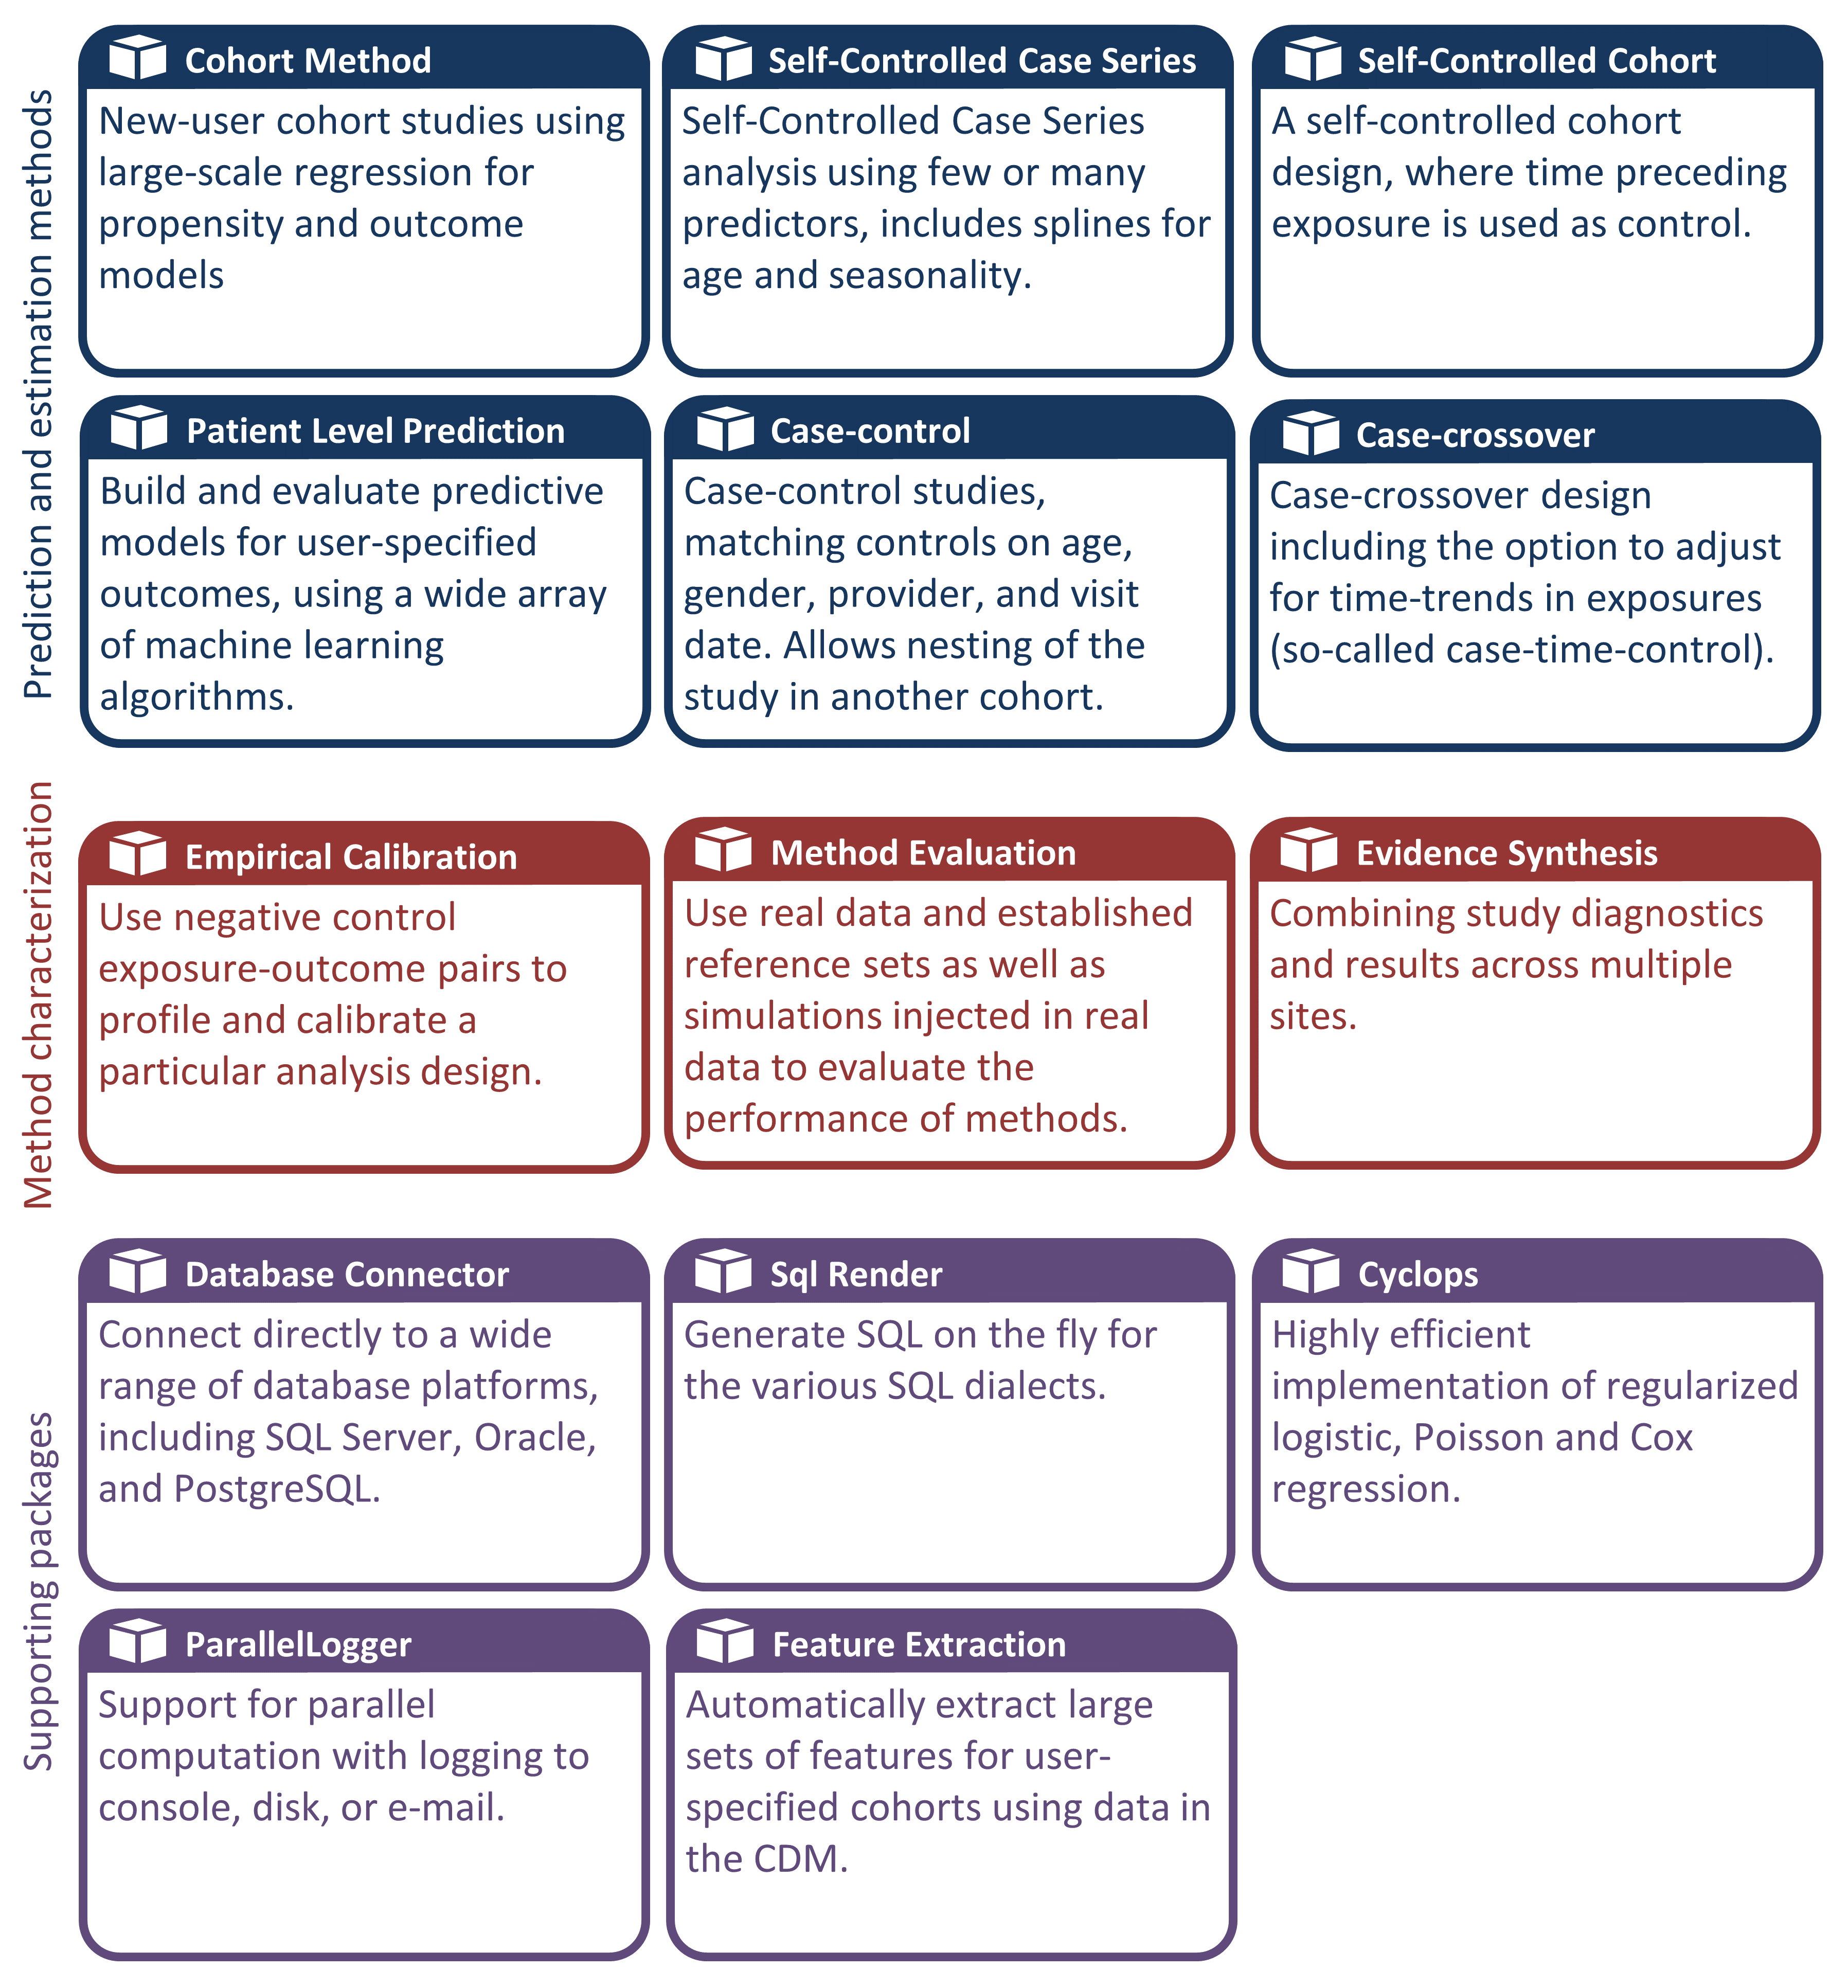
\includegraphics[width=0.50\textwidth]{figures/methodsLibrary.png}
\caption{Biblioteca de Métodos OHDSI. Extraída del Libro de OHDSI \cite{OHDSIbook}}
\label{fig:methodsLibrary}
\end{figure}
    
     Todo ello no solo facilita la tarea del analista de datos sino que además favorece la interoperabilidad entre los estudios, puesto que todos los estudios que utilizan ATLAS implementan (en una capa inferior) los mismos métodos, el mismo lenguaje de programación y la misma estructura de análisis (véase \ref{sec:05Evidencia} ''¿Cómo generar evidencia?''). 

     \item \textbf{Reciclabilidad}. Por último, otro beneficio es que gracias a estas características ATLAS permite diseñar estructuras para el estudio de los datos que puedan utilizarse en diferentes bases de datos distintas. Volviendo al ejemplo de la plancha en \ref{sec:05OHDSI} ''¿Qué es OHDSI?'', esto quiere decir que una misma plancha (o estudio) puede conectarse a cualquier enchufe de cualquier región (a cualquier base de datos). ATLAS está intrínsicamente configurada para diseñar análisis reproducibles, por lo que los elementos que se configuran durante un análisis de datos (grupos de cohortes, estimadores, predictores, grupos de conceptos...) se pueden exportar fácilmente a modo de estructura general e implementarse sobre otro estudio que, aunque posea datos distintos ejecute ATLAS. Por tanto las estructuras más eficientes que se utilizen en un análisis remoto, pueden compartirse en la red de la comunidad y ser utilizados en cualquier nodo y cualquier estudio, favoreciendo la reciclabilidad, reproducibilidad e interoperabilidad del estudio.
    
\end{enumerate}

\subsubsection{Aspectos técnicos}

En cuanto a los aspectos técnicos, ATLAS se despliega como una herramienta basada en web, normalmente alojada en un servidor Apache, combinada con la WebAPI de OHDSI. Generalmente se recomienda su despliegue en Google Chrome. Además la herramienta puede implementarse de forma pública a través de internet o tras el firewall de la red privada de una organización, según las necesidades de la entidad que lo implementa.

Sin embargo, es importante recalcar que tanto ATLAS como la mayoría de las herramientas de OHDSI no consiste en un archivo ejecutable aislado sino en una aplicación contenida y dependiente de un ecosistema completo basado en web. La dependencia principal y red que sostiene a ATLAS es la \textbf{WebAPI}.

\begin{figure}[H]
    \centering
    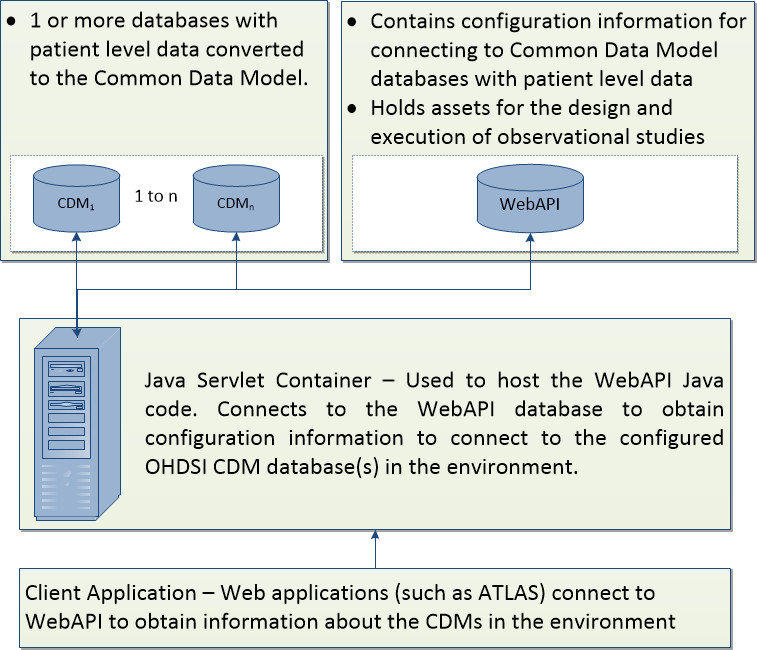
\includegraphics[width=0.700\textwidth]{figures/webAPIwiki.png}
     \caption{Estructura de la WebAPI. Extraída de la wiki de github \cite{githubWebAPIwiki}}.
    \label{fig:webAPIwiki}
\end{figure}

Tal y como se muestra en la Figura \ref{fig:webAPIwiki} ''Estructura de la WebAPI'', la WebAPI es la aplicación que proporciona los servicios RESTful para que la herramienta pueda interactuar con las bases de datos \cite{githubWebAPIwiki}. Por tanto su relación con ATLAS es estrictamente necesaria. ATLAS no es una herramienta aislada sino un eslabón del ecosistema OHDSI.

Por otra parte, la herramienta en sí se muestra a través de una interfaz gráfica, que proporciona un estrecho menú lateral con 15 herramientas para el análisis de datos. La interfaz de la herramienta seleccionada se muestra en el lado derecho, como se muestra en la Figura \ref{fig:ATLASdemoHome} ''Captura de pantalla del menú principal de ATLAS demo''.

\begin{figure}[H]
\centering
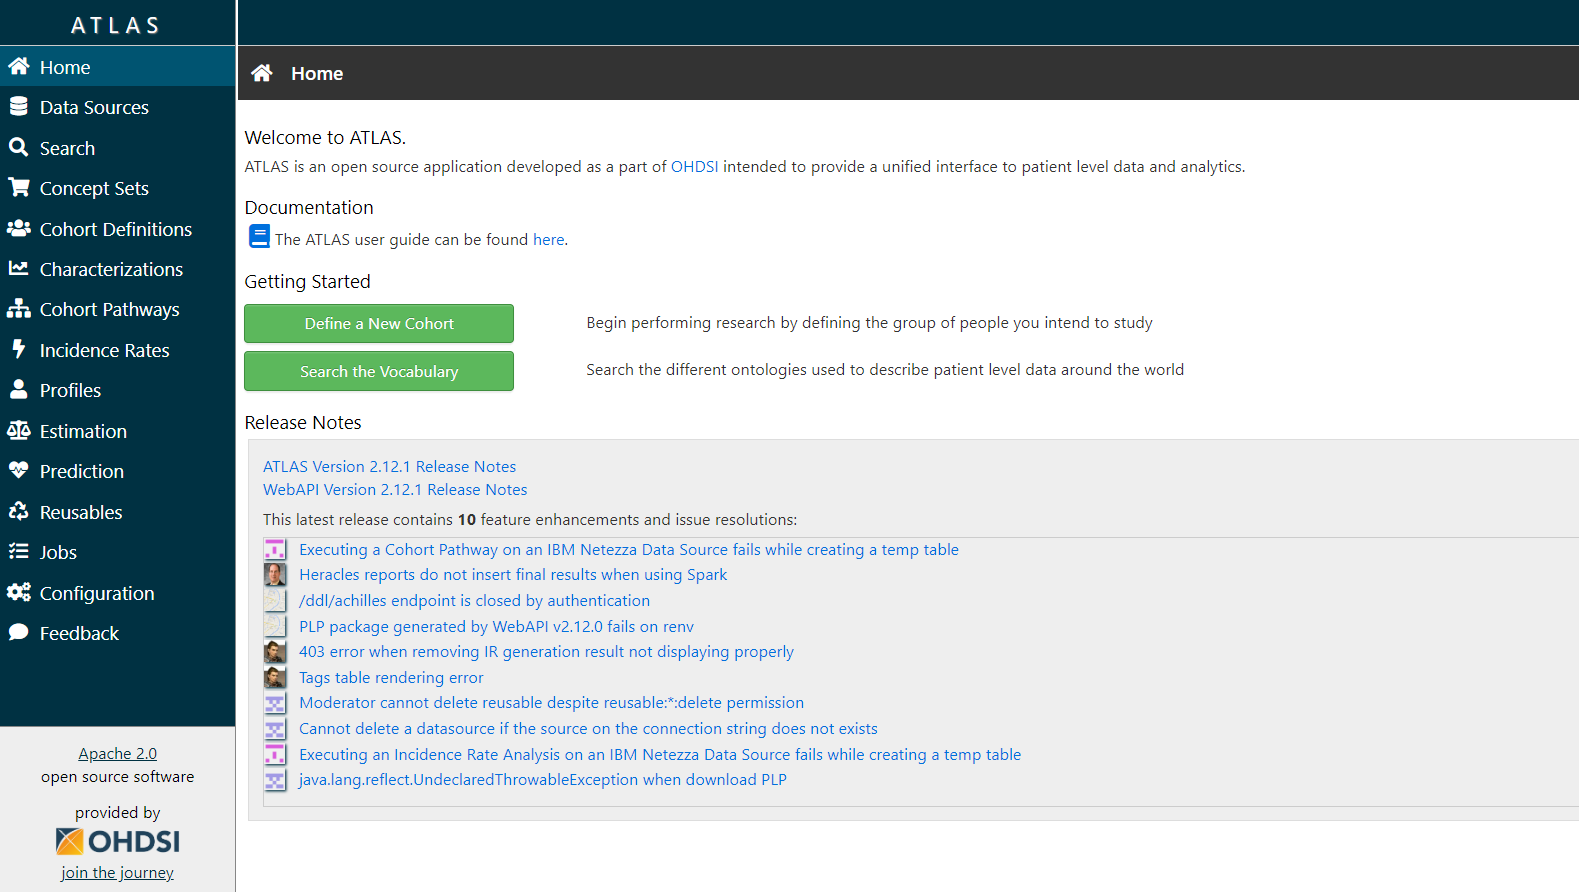
\includegraphics[width=0.90\textwidth]{figures/ATLASdemoHome.png}
     \caption{Captura de pantalla del menú principal de ATLAS demo}
    \label{fig:ATLASdemoHome}
\end{figure}

Recientemente, en diciembre de 2023, ATLAS lanzó su versión 2.14.1 que está en correcto funcionamiento y es la que se utiliza en el desarrollo del Trabajo Fin de Grado. Más información sobre los aspectos técnicos de la herramienta se encuentran en el repositorio de github \cite{githubATLAS}.

\subsubsection{Estrategias de Implementación}

La implementación de ATLAS en una organización puede ser una tarea complicada por su dependencia con la WebAPI, la Biblioteca de Métodos y otras dependencias al ecosistema OHDSI. 

No obstante, la organización ha desarrollado varias iniciativas que facilitan su implementación y accesibilidad, para no crear obstáculos en la promoción del uso de la herramienta. Estas iniciativas se describen a continuación.

\begin{enumerate}[label=\alph*.]

    \item \textbf{ATLAS demo} \cite{ATLASdemo}. En primer lugar, esta es una herramienta muy fácilmente accesible que proporciona la comunidad científica para tomar un primer contacto con la herramienta. En este caso, la herramienta es accesible a través del navegador web, publicamente a través de Internet. Cualquier usuario de internet tiene acceso a la herramienta demo. Se le denomina demo porque se sobreentiende que su uso es principalmente educativo o formativo, aunque verdaderamente ofrece todas las capacidades de la herramienta y los análisis que con ella se realizan, podrían reutilizarse en estudios más complejos o de organizaciones privadas.

    \item \textbf{ATLAS Docker}. Por otro lado, también muy fácilmente implementable se presenta \textbf{Broadsea} \cite{githubBroadsea}, que consiste en la virtualización del ecosistema OHDSI en un multicontenedor Docker. Gracias a la facilidad del uso de las tecnologías Docker, esta forma de implementar el ecosistema es bastante sencilla, permitiendo además añadir nuevas configuraciones más complejas (si fuese necesario) añadiendo o eliminando contenedores. Para realizar la parte práctica de este trabajo se emplea la tecnología Docker de Broadsea para implementar ATLAS. A la herramienta ATLAS desplegada con Broadsea, frecuentemente se le denominará a lo largo del documento \textit{ATLAS Broadsea}. El TFG presenta un documento anexo bastante complejo enteramente dedicado a la instalación, despliegue y configuración del entorno Broadsea (véase anexo \ref{anexo:manual} ''Manual de instalación, despliegue y configuración de ATLAS Broadsea''). Adicionalmente, la arquitectura de Broadsea también se presenta en \ref{subsec:07Broadsea} ''Arquitectura de Broadsea''.

    \item \textbf{ATLAS Amazon Web Services}. Otra alternativa que propone la organziación, en colaboración con Amazon, es la virtualización del ecosistema en el entorno de computación en la nube de Amazon Web Services (AWS). Para ello se ofrecen los entornos \textit{OHDSI-in-a-Box} \cite{githubOHDSIBox} y \textit{OHDSIonAWS} \cite{githubOHDSIAWS}. OHDSI-in-a-Box se crea específicamente como un entorno de aprendizaje y se utiliza en la mayoría de los tutoriales proporcionados por la comunidad OHDSI mientras que OHDSIonAWS es una arquitectura de referencia para entornos OHDSI de clase empresarial, multiusuario, escalables. Por las restricciones intrínsecas al uso de AWS, estas alternativas han sido rechazadas para ser empleadas en el TFG.
    
    \item \textbf{ATLAS Azure}. Por último, \textit{OHDSI on AZURE} \cite{OHDSIonAzure} es otra alternativa de virtualización pero a través de la plataforma Microsoft de Azure. No obstante, esta alternativa es la menos común.
    
\end{enumerate}

\subsubsection{Herramientas embebidas}

Si bien las herramientas del ecosistema de OHDSI no son totalmente aisladas, ATLAS presenta en su propia interfaz acceso a dos de estas herramientas de forma íntegra, para facilitar la eficiencia y rapidez en el análisis. Estas herramientas son las siguientes:

\begin{itemize}

    \item \textbf{ACHILLES} \cite{githubACHILLES}. Esta herramienta, de las siglas \textit{Automated Characterization of Health Information at Large-Scale Longitudinal Evidence Systems}, en español Caracterización automatizada de la información sanitaria en sistemas de evidencia longitudinal a gran escala, sirve para caracterizar y/o obtener un reporte estadístico de la base de datos estandarizada que se va a utilizar para el estudio. Intrínsicamente es una librería de R que se implementa como una opción del menú lateral \textit{Data Sources} de ATLAS.
    \item \textbf{ATHENA} \cite{githubATHENA}. Esta herramienta sirve para realizar búsquedas dinámicas en el Vocabulario de OMOP (véase \ref{subsec:07vocab} ''El Vocabulario''). Está implementada en ATLAS en la opción \textit{Search} del menú lateral. Además, se puede acceder a ella online de forma externa a través de su propia página web \cite{ATHENAweb}.
    
\end{itemize}


\subsection{Otras herramientas} \label{subsec:07otrasHerramientas}

El ecosistema de OHDSI presenta gran cantidad de herramientas adicionales. A continuación se presentan otras herramientas que aunque no se utilizan directamente, son importantes para realizar un análisis de datos completo. 

\begin{itemize}
    
    \item \textbf{HADES} \cite{githubHADES}. HADES, del inglés\textit{ Health Analytics Data-To-Evidence Suite} y en español Suite de análisis sanitario de datos a evidencia, es el nombre con el que se denomina a la herramienta que implementa el paquete R con la Biblioteca de Métodos de OHDSI (ver Figura \ref{fig:methodsLibrary} ''Biblioteca de Métodos OHDSI''). Se puede instalar como un entorno independiente mediante Java y Rtools para implementar análisis mediante código estandarizado (véase Figura \ref{fig:analysisImplementations} ''Tres vías para la implementación de un análisis observacional''). No se utiliza en el TFG más alla de la implementación subyacente de las bibliotecas en ATLAS.
    \item \textbf{Rabbit tools y Usagi} \cite{OHDSIsoftTools}. Estas herramientas en conjunto llevan a cabo el proceso de ETL, para omopizar las bases de datos al Modelo de Datos Común de OMOP. Las herramientas son tres: White-Rabbit, Rabbit-In-Hat y Usagi. No se utiliza directamente en el TFG porque el dataset utilizado para el análisis ya estaba previamente omopizado.
    \item \textbf{Data Quality Dashboard} \cite{githubDQD}. Esta herramienta, en español Panel de control de calidad de los datos, pertenece a un paquete de HADES aunque implementado como una interfaz gráfica aparte para facilitar su acceso online. Tal y como su nombre indica sirve para automatizar la tarea de comprobación de la calidad de los datos, un paso previo fundamental antes de realizar un análisis de datos. Tampoco se utiliza directamente para el TFG porque este estudio se llevó a cabo durante la omopización del dataset.
        
\end{itemize}

\section{Programas informáticos empleados} \label{sec:07programas}

Los programas informáticos que han permitido el despliegue de este entorno tecnológico que envuelve al sistema son los siguientes:  Google Chrome, Docker, PostgreSQL y Github.


\subsubsection{Google Chrome}

Google Chrome es el navegador web de Google que permite el acceso a internet y la búsqueda en la web a través de una interfaz amigable e intuitiva \cite{GoogleChrome}. 

Chrome es el navegador recomendado por OHDSI para desplegar las herramientas de su ecosistema y más especialmente en el despliegue de Broadsea, permitiendo el acceso al servidor donde se aloja el sistema. Por tanto su uso ha sido muy relevante como portal de acceso a las herramientas OHDSI.


\subsubsection{Docker}

Docker es una plataforma abierta para desarrollar, enviar y ejecutar aplicaciones. Docker le permite separar sus aplicaciones de su infraestructura para que pueda entregar software rápidamente. Con Docker, puede administrar su infraestructura de la misma manera que administra sus aplicaciones \cite{DockerWebsite}.

De esta forma, Docker permite empaquetar y ejecutar aplicaciones en contenedores, entornos poco aislados pero seguros. Esto posibilita la ejecución de múltiples contenedores simultáneamente en un mismo host, sin depender de lo instalado en él. Los contenedores son ligeros y contienen todo lo necesario para la aplicación, facilitando su compartición y asegurando consistencia entre usuarios. 

El uso de Docker en el desarrollo del proyecto es evidente, es la herramienta que despliega Broadsea y, por consiguiente, ATLAS. El proceso concreto de instalación, despliegue y configuración de Docker así como la explicación detallada de su estructura y archivos más importantes se presenta en el anexo \ref{anexo:manual} ''Manual de instalación, despliegue y configuración de ATLAS Broadsea''.

\subsubsection{PostgreSQL}

PostgreSQL es un potente sistema de base de datos relacional de objetos de código abierto que utiliza y amplía el lenguaje SQL combinado con muchas funciones que almacenan y escalan de forma segura las cargas de trabajo de datos más complicadas \cite{PostgreWebsite}.

El uso de postgre es fundamental para la implementación correcta de Broadsea, puesto que su base de datos se implementa según PostgreSQL. Las bases de datos externas que se interactúan con la WebAPI pueden estar en otros lenguajes relacionales, pero el sistema de Broadsea intrínsicamente solo se sostiene sobre Postgre.

El proceso concreto de instalación, despliegue y configuración de la base de datos Postgre se realiza a través de la interfaz visual de pgAdmin 4.0 \cite{pgAdminWebsite} y la explicación detallada de su estructura y archivos más importantes se presenta en el anexo \ref{anexo:manual} ''Manual de instalación, despliegue y configuración de ATLAS Broadsea''.

\subsubsection{Github}

GitHub es una plataforma para desarrolladores que les permite crear, almacenar, gestionar y compartir su código. Utiliza el software Git, proporcionando control de versiones distribuido, además de control de acceso, seguimiento de errores, solicitudes de funciones de software, gestión de tareas, integración continua y wikis para cada proyecto \cite{GithubWikipedia}.

El uso de Github es muy recomendado debido a que la mayor parte de la información sobre OHDSI y sus herramientas se encuentran en internet disponibles en repositorios de Github (véase \ref{sec:05OHDSI} ''¿Qué es OHDSI?''). 

Además, siguiendo esta iniciativa de OHSI, para desarrollar este Trabajo Fin de Grado se ha creado un repositorio de Github específico \cite{vallealonsodc} que contiene toda la documentación relevante a su desarrollo (archivos latex, pdf...) y archivos de variables de entorno o scripts utilizados durante la configuración del entorno del sistema o la realización del análisis de datos.   


\section{Conclusiones} \label{sec:07conclusiones}

En esta sección se concluye que el entorno de trabajo del proyecto está enmarcado en el entorno de estándares y herramientas de la organización OHDSI, desplegados a través de una serie de programas informáticos. 

Conocer el entorno de trabajo del proyecto y de OHDSI es gran relevancia puesto que no puede entenderse ATLAS sin conocer estos otros. 
